\section{Mixed strategies and Nash equilirbia in dynamic games, subgame-perfect Nash equilibria}

\Que{What is the difference between mixed and behavioral strategies? Under what condition are the two concepts equivalent?}
\Ans[Mixed strategies]{ are decided before the game starts; \textbf{behavioral}, on the other hand, are more "realistic" and every move is decided after opponent makes his (more formally: at each information set, select a random move from your set of available moves). They are equivalent under the perfect \textbf{recall assumption}: players do not forget the information they have acquired.}

\Que{How do you find the solution(s) of a sequential game?}
\Ans[By backward induction:]{ starting from the leaf with maximum payoff for the player, replace the parent node with the payoff, repeat until root.
More formally:
\begin{itemize}
    \item Start from the leaves of the tree
    \item Partition them according to their parent node (which is a move of some player $i$)
    \item For each set in the partition, find the leaf $x_j$ with maximum payoff for player $i$
    \item Add the corresponding branch to player $i$’s strategy
    \item Replace the parent node with the payoff of $x_j$
    \item Repeat until the root is reached
\end{itemize}
Solutions can be unique as can be more than one. This way, we find the \textbf{equilibrium path}.}
\Spec[A (proper) \textbf{subgame} $\ml{G'}$ of a game $\ml{G}$ contains a single node of the tree and all of its descendants, with the requirement that
\mat{x_j \in \ml{G'}, x_j \in h_i \hookrightarrow x_k \in \ml{G'} \fa x_k \in h_i}

An \textbf{equilibrium path} is a path that contains all nodes of a NE alont the tree rapresentation of the game.]

\Que{What is a subgame-perfect NE? In which cases is a NE not subgame-perfect?}
\Ans[A subgame-perfect NE (SPE)]{ is the strategy that yield a NE in every subgame. Every SPE is a NE in the parent game and every finite dynamic game has at least one SPE. This means that every sequential game (tic tac toe, chess etc \dots) has a NE.}

\Que{\textbf{Exercise}

\textit{Solution can be found in Lecture13 pdf}

It is the discount sales season, Karen (K) and Lou (L) wants to go shopping. He thinks it is best to wait until the last three days of the discount sales, because prices are cheapest. On day 1, Lou asks Karen (K) to go with him. If Karen says yes (Y), they go shopping and the game ends. If Karen says no (N), Lou can either give up (G) or request (R) again the following day. On day 2, the same happens. On day 3, if K still says N, the game ends as well and does not go into a further day. If in the end K and L do not go shopping, both of their payoffs are 0. If they do, their payoffs are computed as $u_K = d$ and $u_L = 5 - 2d$, respectively, where $d$ is the day in which they go. All of this information about the game is common knowledge among the players.
\begin{enumerate}
    \item Represent the game in its extensive form.
    \item  How many (pure) strategies do K and L have, respectively?
    \item  Find the SPE of this game.
    \item  Find one NE that is not subgame-perfect.
    \item  Represent the game in its normal form.
    \item  Find all the NE of this game (both SPE and non-SPE).
\end{enumerate}
}
\Ans[Solution]{
\begin{enumerate}
    \item 
    \begin{figure}[!ht]
        \centering
        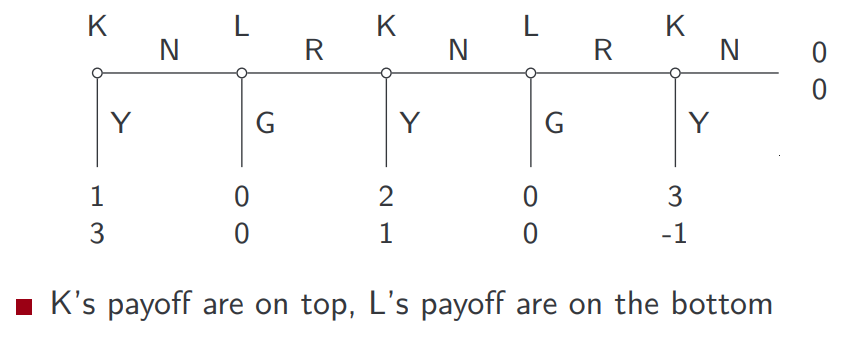
\includegraphics[width=0.5\linewidth]{ex12-1.png}
    \end{figure}

    \item K plays in 3 information sets and has 2 possible actions in each set: $2^3 = 8$ possible strategies. Her strategies are triplets: \m{s_K = (a_0, a_2, a_4), a_j \in {Y, N}}
    
    L plays in 2 information sets has 2 possible actions in each set: $2^2 = 4$ possible strategies. His strategies are triplets: \m{s_L = (a_1, a_3), a_j \in {G, R}}
    \item The SPE can be found via backward induction. On the last day, K prefers Y (payoff 3) to N (payoff 0): $a_4 = Y$. Before that, L prefers G (payoff 0) to R (payoff -1, knowing K’s next choice): $a_3 = G$. Before that, K prefers Y (payoff 1) to N (payoff 0, knowing how the rest of the game will play out): $a_2 = Y$. Only SPE: $s_K = (N, Y , Y )$, $s_L = (R, G)$
    \item Just chose and irrational move on SPE (outside equilibrium path)
    \item Just draw it
    \item Trivial and left to the reader
\end{enumerate}
}